\documentclass[12pt,a4paper]{article}
\usepackage[utf8]{inputenc}
\usepackage[german]{babel}
\usepackage[T1]{fontenc}
\usepackage{amsmath}
\usepackage{amsfonts}
\usepackage{amssymb}
\usepackage{graphicx}
\usepackage[left=2.5cm,right=2.5cm,top=2cm,bottom=2cm]{geometry}
\usepackage{float}
\author{Gruppe C14 \\ Julián Häck, Martin Koytek, Lars Wenning, Erik Zimmermann}
\begin{document}
\section{z.B. Widerstand, Teilversuch 4.1}
\subsection{Versuchsbeschreibung}
Aus dem Ohm'schen Gesetz folgt:
\[R=\frac{U}{I}\]
Aus der am Widerstand anliegenden Spannung $U$ und dem durch den Widerstand fließenden Strom $I$ wird hier der Wert für den Widerstand $R$ berechnet.
\subsection{Versuchsaufbau und Durchführung}
%Genaue Beschreibung der verwendeten Aufbauten unter Verwendung von Skizzen oder Photos
%Beschreibung der Messwerterfassungseinstellungen (eingestellte %Messzeiten, Messbedingungen,
%Trigger, Anzahl der Messungen) und der Durchführung der Versuche. (max. 1 Seite)
\begin{center}
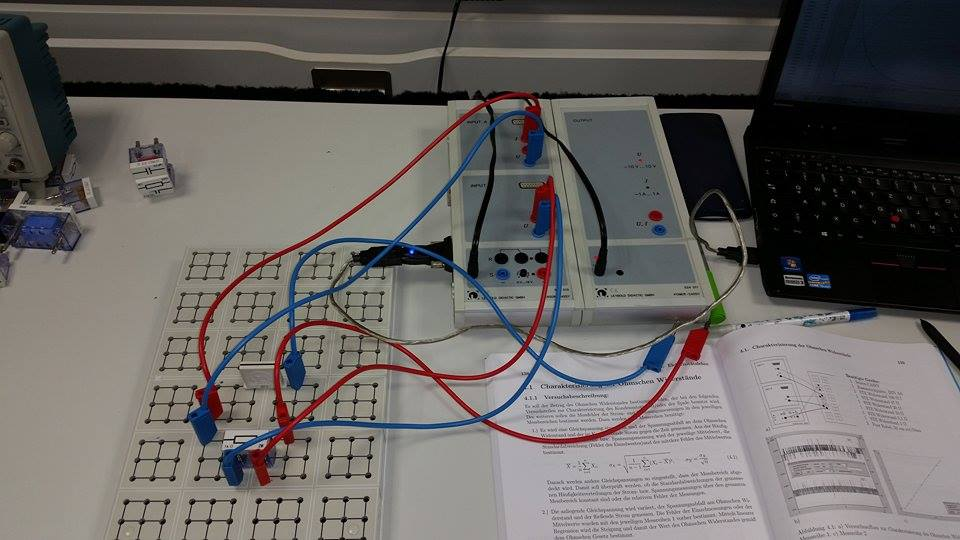
\includegraphics[scale=0.35]{12000155_1207085929316467_1534534399_n.jpg}
\end{center}

Der erste Versuch bestand aus Rauschmessungen in denen jeweils die Spannung $U$ und der Strom $I$ bei konstanten Spannungen aufgezeichnet wurde.
Bei den Messungen wurden jeweils 1000 Werte über einen Messzeitraum von von $10ms$ aufgezeichnet. Die Spannung wurde in einem Messbereich von $-10V$ bis $+10V$ und der Strom von $-0,1A$ bis $+0,1A$ gemessen.
Anschließend wurde die Spannung variiert um den Messbereich abzudecken und eine eventuelle relative Abhängigkeit des Fehlers von der Spannung auszuschließen. 

\subsection{Versuchsauswertung}
Aus den Daten der Strom- und Spannungsmessung wurden anschließend die Mittelwerte von $U$ und $I$ mit deren statistischen Fehler bestimmt.
Die statistischen Fehler wurden dann mittels Fehlerfortpflanzung der aus den Herstellerangaben entnommenen $\sigma_{U,sys}$ und $\sigma_{I,sys}$ errechnet. 
Aus den jeweils berechneten Werten für $R$ konnte dann der Mittelwert und damit das Endergebnis angegeben werden.
\subsubsection{Rohdaten}
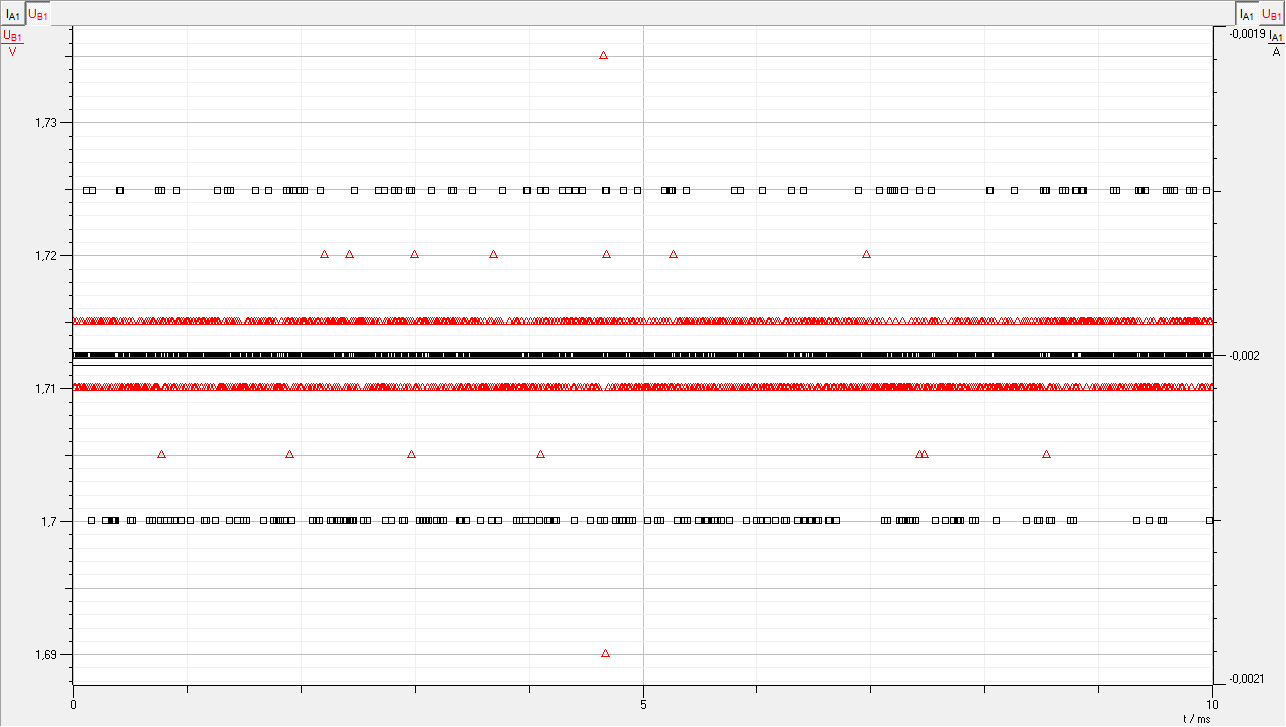
\includegraphics[scale=0.6]{Rauschmessung1.png}
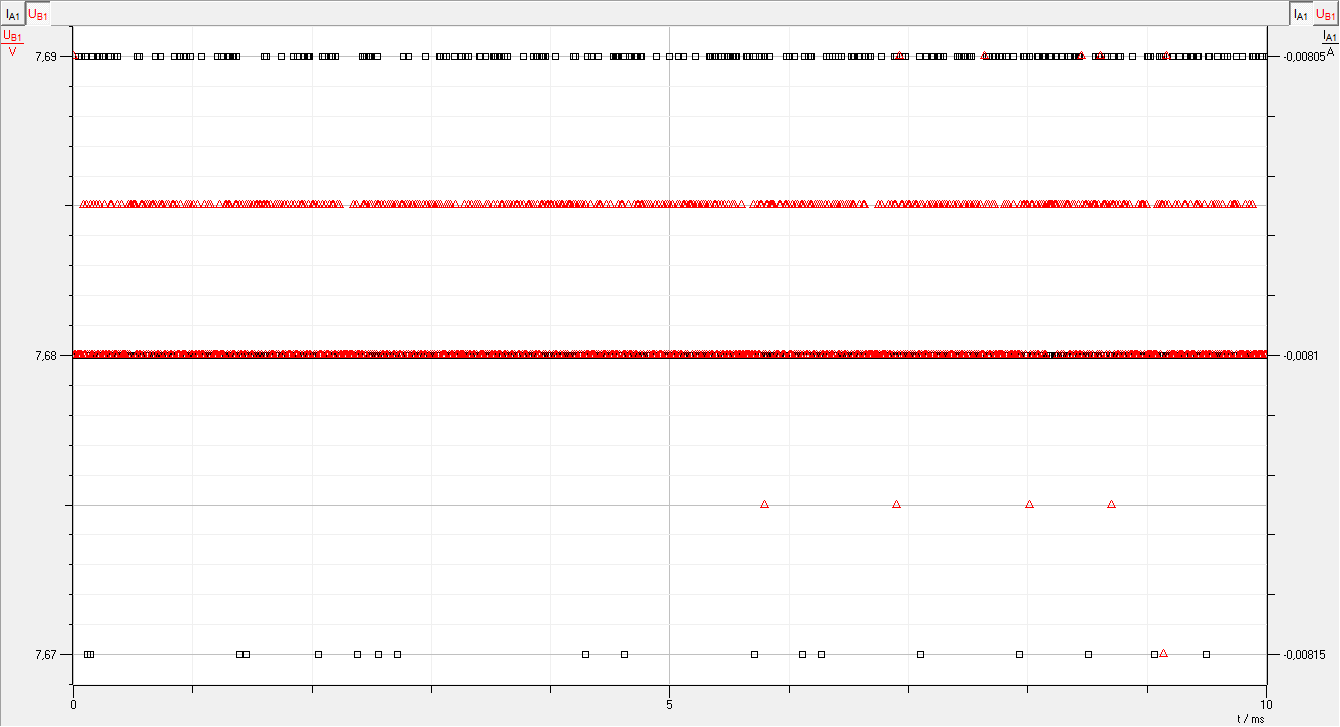
\includegraphics[scale=0.575]{Rauschmessung2.png}  
\newpage
\subsubsection{Analyse}
%Analyse der Daten inklusive Fehlerrechnung Residuen und Pullverteilung. (1 Seite)
Formeln:
\begin{align*}
R=\frac{\bar{U}}{\bar{I}} \hspace{2cm} 
\sigma_R=\sqrt{(\frac{1}{\bar{I}})^{2} \cdot \sigma_{\bar{U}}^{2}+(\frac{\bar{U}}{\bar{I}^2})^{2} \cdot \sigma_{\bar{I}}^{2}} \hspace{2cm}\frac{\sigma_R}{R}=\sqrt{(\frac{\sigma_{\bar{U}}}{\bar{U}})^2+(\frac{\sigma_{\bar{I}}}{\bar{I}})^2}
\end{align*}
Aus den Fehlerrechnungen der statistischen Fehlern aus der Messung und den systematischen Fehlern aus den Herstellerangaben des Sensor-Cassy berechneten wir folgende Werte für R:
\begin{table}[H]\centering
\caption{1. Messung}
\begin{tabular}{c|c|c|c|c|c|c}
$\bar{U}$& $\sigma_{\bar{U}}$& $\bar{I}$& $\sigma_{\bar{I}}$& $R$& $\Delta R_{stat}$& $\Delta R_{sys}$ \\ \hline
$1.71V$& $0.00009V$& $0.002A$& $0.00002A$& $855\Omega$& $8.55\Omega$& $233.27\Omega$\\ 
$3.88V$& $0.00008V$& $0.004A$& $0.00002A$& $970\Omega$& $4.85\Omega$& $135.8\Omega$\\ 
$5.82V$& $0.00007V$& $0.006A$& $0.00003A$& $970\Omega$& $4.85\Omega$& $101.84\Omega$ \\
$7.68V$& $0.00009V$& $0.008A$& $0.000026A$& $960\Omega$& $2.4\Omega$& $74\Omega$ \\
\end{tabular} 
\end{table}
%\subsubsection{Fazit}
%Diskussion der Ergebnisse und Vergleich der erzielten Ergebnisse mit theoretischen %Vorhersagen.
%(1 Seite)
\end{document}